\documentclass[sigconf, nonacm]{acmart}

%%% do not modify the following VLDB block %%
%%% VLDB block start %%%
\usepackage{pvldb}% VLDB/PVLDB formatting overrides, see pvldb.sty for details.
%%% VLDB block end %%%

\renewcommand\vldbdoi{XX.XX/XXX.XX}
\renewcommand\vldbpages{XXX-XXX}
\renewcommand\vldbavailabilityurl{https://github.com/sanmish4ds/HyperVectorOptimizer}

\usepackage{booktabs}
\usepackage{array}
\usepackage{tikz}
\usepackage{pgfplots}
\pgfplotsset{compat=1.18}
\usetikzlibrary{arrows.meta,positioning,shapes.geometric,calc}
\setlength{\emergencystretch}{3em}

% Every experimental number below is generated from results/*.json by experiments/make_tables.py.
\input{generated/numbers}
\input{generated/figdata}

\newcommand{\sg}{s_g}
\newcommand{\sloc}{s_{\text{loc}}}
\newcommand{\Ppre}{\Pi_{\text{pre}}}
\newcommand{\Pfus}{\Pi_{\text{fused}}}
\newcommand{\Ppost}{\Pi_{\text{post}}}

\begin{document}
\title{It's Not How Many, It's Where: Local-Selectivity Plan Routing for Filtered Vector Search}

\author{Sanjay Mishra}
\affiliation{%
  \institution{Independent Researcher}
  \city{Raleigh}
  \state{NC}
  \country{USA}
}
\email{sanmish4@icloud.com}

\begin{abstract}
A filtered vector query asks for the items most similar to a query, but only among those that satisfy a condition, such as ``the ten papers closest to this one, published in physics''. A database can answer it in three ways: filter first and then compare vectors, search a similarity graph and then filter, or filter during the graph search. The fastest choice varies sharply from query to query. Today's optimizers decide mainly from \emph{how many} rows match the filter. We show that what matters is \emph{where} the matching rows are. If they lie near the query, a graph search finds them quickly; if they lie far away, the search wastes time and filtering first is faster. For example, two real arXiv queries whose filters each match about $6\%$ of the table need opposite plans: the plan that is best for one is $\ExBGlobalSlowdown\times$ slower than necessary for the other.

We present \emph{HyperVector-Optimizer} (HVO). HVO estimates how far a search must travel to find enough matches, using a small summary of the data that never touches the index, and then picks the plan that is safest given its uncertainty. HVO runs both in a standalone benchmark and inside PostgreSQL with \texttt{pgvector}. On one million arXiv papers, it cuts mean latency by $\GainHvoC\%$ (95\% CI $\GainLoHvoC$--$\GainHiHvoC\%$) compared with the best tuned rule based on filter size, and reduces tail latency up to fourfold. On Amazon products and synthetic data, the gain in mean latency is not statistically clear. In PostgreSQL, \texttt{pgvector} with default settings reaches a mean recall of only $\PGStockRecC$ on arXiv (it returns about half of the correct results); HVO returns more correct results than forcing \texttt{pgvector}'s iterative scan on every query, and is faster. We release the code and both real benchmarks.
\end{abstract}

\maketitle

%%% do not modify the following VLDB block %%
%%% VLDB block start %%%
\vldbtopmatter
%%% VLDB block end %%%

\section{Introduction}\label{sec:intro}
Search applications increasingly ask a database for items that are similar to something, but only among items that meet some conditions. A chatbot may look for documents similar to a question, but only from a certain team; a shop may look for products similar to one a customer viewed, but only in stock and under a price limit~\cite{wei2020analyticdbv,zhang2023vbase,patel2024acorn,amanbayev2026fanns}. Each item is stored as an \emph{embedding}---a list of numbers that captures its meaning---next to ordinary columns such as category or year. A typical query asks for the ten papers most similar to a given one, but only among published physics papers:
\begin{center}
\footnotesize
\begin{tabular}{@{}l@{}}
\texttt{SELECT id FROM papers}\\
\texttt{WHERE published AND archive IN ('physics', ...)}\\
\texttt{ORDER BY embedding <\#> q LIMIT 10;}
\end{tabular}
\end{center}
In general, such a query combines range conditions, \texttt{IN} lists and conditions on a joined table with an ordering by similarity to the query vector $\mathbf{q}$, and asks for the top $k$ results.

Many systems support such queries. Some are ordinary databases that store embeddings next to regular columns, such as PostgreSQL with \texttt{pgvector}~\cite{pgvector2024} or DuckDB with \texttt{vss}~\cite{duckdbvss2024}. Others are dedicated vector databases, such as Milvus~\cite{wang2021milvus}. In every system, there are three basic ways to answer the query:
\begin{itemize}
    \item \emph{Filter first} ($\Ppre$). Find every row that passes the filter, compare each one with the query, and keep the closest $k$. This always gives the exact answer, but it may compare tens of thousands of rows to return just ten.
    \item \emph{Search first} ($\Ppost$). Use a similarity index (HNSW~\cite{malkov2018hnsw}) to visit rows in order of similarity, starting with the closest, and check each against the filter until $k$ have passed. This is how \texttt{pgvector}'s iterative scan and VBase~\cite{zhang2023vbase} work. It is very fast when matching rows are close to the query, but slow when they are far away, and it can miss some answers.
    \item \emph{Filter while searching} ($\Pfus$). Walk the index as before, but step only onto rows that pass the filter~\cite{patel2024acorn,wang2021milvus}. This is often fast, but it can miss answers when few matching rows lie near the query.
\end{itemize}

The best choice can differ greatly from one query to the next. Figure~\ref{fig:example} shows two real queries from our arXiv benchmark. Query~A looks for the ten papers most similar to a computer-science paper, \emph{``\ExATitle''}, but only among physics papers. Query~B looks for the ten papers most similar to a physics paper, \emph{``\ExBTitle''}, but only among published physics papers. Both filters keep about $6\%$ of the one million papers ($\ExASg\%$ and $\ExBSg\%$). Database optimizers choose a plan mainly from this kind of number: the share of rows that pass the filter. A rule based only on this share must treat the two queries the same way. The best such rule we could tune filters both first. That is the right choice for Query~A ($\ExATPre$\,ms), but $\ExBGlobalSlowdown$ times too slow for Query~B, which searching first answers in just $\ExBTPost$\,ms. No rule based only on \emph{how many} rows match can get both queries right (Section~\ref{sec:understanding}).

What separates the two queries is not how many papers match, but \emph{where} they are. A paper on dialogue generation sits among computer-science papers, far from physics papers. A paper on epidemics, filed under physics, sits among physics papers. A search that starts at the query and moves outward is cheap when matching papers are nearby and expensive when they are far away. For Query~B, the search passes only $\ExBHk$ papers before it has found ten matches; for Query~A it must pass $\ExAHk$. We call the share of rows that pass the filter the \emph{global selectivity}, and $k$ divided by the number of rows the search must pass the \emph{local selectivity}. Both queries have a global selectivity of about $6\%$, but the local selectivity is $\ExBSloc\%$ for Query~B and only $\ExASloc\%$ for Query~A.

Recent work recognizes that global selectivity is not enough. Exqutor estimates how many results a vector search will find by probing the index or by sampling~\cite{exqutor2026}, and benchmark studies show that performance swings widely when filters and similarity are related~\cite{amanbayev2026fanns,iff2025benchmark,shi2025unified}. Three questions remain open: how to define the local selectivity that decides the plan, how to estimate it quickly without touching the index, and how to choose a plan safely, inside a real database, when the estimate is wrong.

This paper presents \emph{HyperVector-Optimizer} (HVO), which chooses each query's plan from its local selectivity. HVO estimates local selectivity with a small summary of the data, the \emph{Polytope-Ball Sketch} (HPBS), without touching the index. It predicts each plan's running time from measurements taken on the actual machine, and it picks the plan that stays fast even if its estimate is somewhat wrong. For Query~A, HVO estimates $\ExAEstCal\%$ (true: $\ExASloc\%$) and filters first; for Query~B it estimates $\ExBEstCal\%$ (true: $\ExBSloc\%$) and searches first. Both are the fastest plans that return the correct answer. We also prove that HVO never sends a query whose best plan is filtering first to a slower plan, as long as its uncertainty range covers the true value, and that any rule based only on global selectivity can become arbitrarily slow as the table grows.

We test HVO on two real datasets, one million arXiv papers and one million Amazon products, and on two synthetic ones. To know the best plan for certain, we run every plan for every test query. Figure~\ref{fig:example} is not a rare case: on the arXiv queries, HVO and the best global rule choose different plans for $\DisagreeC\%$ of queries, and HVO's choice is faster in $\HvoFasterDisagreeC\%$ of those. Overall, HVO cuts average query time on arXiv by $\GainHvoC\%$ (95\% confidence interval $\GainLoHvoC$--$\GainHiHvoC\%$) and cuts the time of the slowest queries by up to four times. On Amazon it speeds up the slowest queries, but its gain in average time is not statistically clear; on synthetic data the averages tie. Inside PostgreSQL, \texttt{pgvector} with default settings and Exqutor reach a mean recall of only about $\PGStockRecC$ on these queries, returning about half of the correct results. HVO returns more correct results than forcing \texttt{pgvector}'s iterative scan on every query, and is faster. HVO does not help when only one result is requested ($k=1$), because planning then takes longer than the query itself.

\noindent\textbf{Our contributions are:}
\begin{itemize}
  \item \textbf{Local selectivity.} A definition of local selectivity based on the $k$-th match, and a sketch that estimates it without touching the index (Sections~\ref{sec:example} and~\ref{sec:sketch}).
  \item \textbf{Robust plan choice.} A way to choose plans safely using measured costs, with proven guarantees (Sections~\ref{sec:costs}--\ref{sec:theory}; proofs in the extended version~\cite{hvoextended}).
  \item \textbf{PostgreSQL integration.} HVO as a planner extension for PostgreSQL and \texttt{pgvector} (Section~\ref{sec:pg}).
  \item \textbf{Evaluation and benchmarks.} An evaluation in which every plan runs for every query, and two real-data benchmarks released with exact answers~\cite{hvobench} (Section~\ref{sec:eval}).
\end{itemize}

\begin{figure*}[!t]
\centering
\begin{minipage}[t]{0.485\textwidth}
\centering
\begin{tikzpicture}
\node[draw=gray!60, rounded corners=2pt, fill=gray!5, text width=0.93\textwidth, align=left, font=\scriptsize, inner sep=4pt, minimum height=2.15cm] {\textbf{Query A} \hfill anti-correlated ($\rho_{\text{GLS}}=\ExARho$)\\[2pt]
Ten papers closest to \emph{``\ExATitle''} (\texttt{\ExAPrimary}), where \ExAFilter\\[3pt]
$s_g=\ExASg\%$,\quad $s_{\text{loc}}=\ExASloc\%$,\quad $h_k=\ExAHk$};
\end{tikzpicture}\\[2pt]
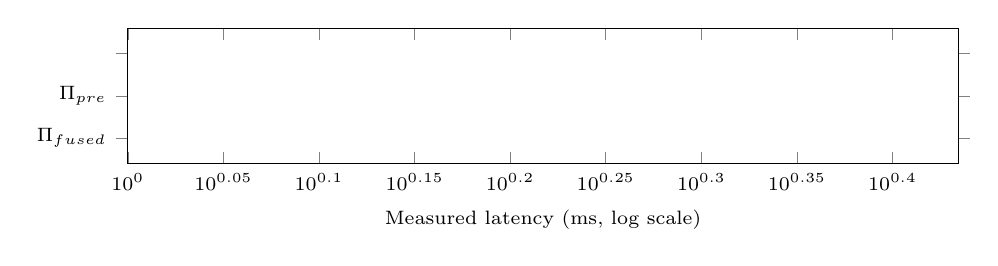
\begin{tikzpicture}
\begin{axis}[
    width=\textwidth, height=3.3cm,
    xbar, xmode=log, log origin x=infty, xmin=0.05, xmax=400, bar width=7pt,
    symbolic y coords={post,fused,pre}, ytick=data,
    yticklabels={$\Ppost$, $\Pfus$, $\Ppre$},
    xlabel={Measured latency (ms, log scale)}, xlabel style={font=\scriptsize}, ticklabel style={font=\scriptsize},
    nodes near coords, nodes near coords style={font=\tiny, anchor=west}, point meta=explicit symbolic,
    enlarge y limits=0.3]
\addplot[fill=gray!35, draw=gray!70] coordinates {(\ExATPost,post) [\ExATPost\,ms, recall \ExARecPost] (\ExATFused,fused) [\ExATFused\,ms, recall \ExARecFused] (\ExATPre,pre) [\ExATPre\,ms, exact\quad$\leftarrow$ \textcolor{red!65!black}{global rule}, \textcolor{green!40!black}{HVO}]};
\end{axis}
\end{tikzpicture}
\end{minipage}\hfill
\begin{minipage}[t]{0.485\textwidth}
\centering
\begin{tikzpicture}
\node[draw=gray!60, rounded corners=2pt, fill=gray!5, text width=0.93\textwidth, align=left, font=\scriptsize, inner sep=4pt, minimum height=2.15cm] {\textbf{Query B} \hfill positively correlated ($\rho_{\text{GLS}}=\ExBRho$)\\[2pt]
Ten papers closest to \emph{``\ExBTitle''} (\texttt{\ExBPrimary}), where \ExBFilter\\[3pt]
$s_g=\ExBSg\%$,\quad $s_{\text{loc}}=\ExBSloc\%$,\quad $h_k=\ExBHk$};
\end{tikzpicture}\\[2pt]
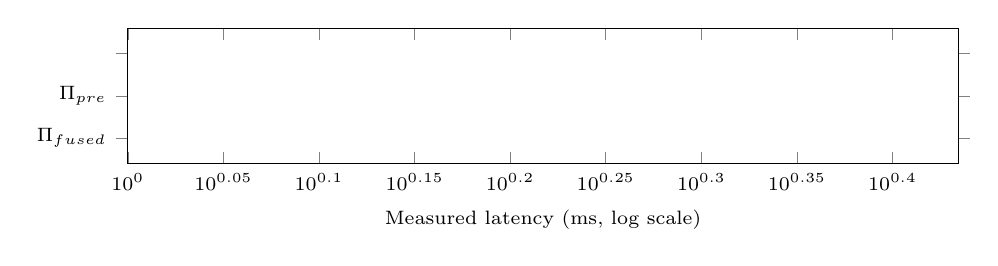
\begin{tikzpicture}
\begin{axis}[
    width=\textwidth, height=3.3cm,
    xbar, xmode=log, log origin x=infty, xmin=0.05, xmax=400, bar width=7pt,
    symbolic y coords={post,fused,pre}, ytick=data,
    yticklabels={$\Ppost$, $\Pfus$, $\Ppre$},
    xlabel={Measured latency (ms, log scale)}, xlabel style={font=\scriptsize}, ticklabel style={font=\scriptsize},
    nodes near coords, nodes near coords style={font=\tiny, anchor=west}, point meta=explicit symbolic,
    enlarge y limits=0.3]
\addplot[fill=gray!35, draw=gray!70] coordinates {(\ExBTPost,post) [\ExBTPost\,ms, exact\quad$\leftarrow$ \textcolor{green!40!black}{HVO}] (\ExBTFused,fused) [\ExBTFused\,ms, exact] (\ExBTPre,pre) [\ExBTPre\,ms, exact\quad$\leftarrow$ \textcolor{red!65!black}{global rule}]};
\end{axis}
\end{tikzpicture}
\end{minipage}
\caption{A real example from the ARXIV-384 benchmark ($k=10$). The two filters match about the same share of the table, so a router that sees only global selectivity sends both queries to the same plan (here filter first, because both are below its tuned threshold of $\ExThreshold\%$). Query~B's matches surround the query paper, and searching first answers it $\ExBGlobalSlowdown\times$ faster; Query~A's matches lie far away, and searching first must pass $\ExAHk$ papers. HVO estimates the local selectivity and routes both queries to their fastest plan that returns the correct answer. ``recall'': share of the true top~10 returned by the graph plans. The pair was selected from the test split by a fixed rule to illustrate the failure mode (Section~\ref{sec:example}); Section~\ref{sec:eval} reports how often it occurs.}
\label{fig:example}
\end{figure*}

\section{Background and Related Work}\label{sec:related}
\emph{Databases with vector search.} Several engines combine vector search with ordinary queries. AnalyticDB-V~\cite{wei2020analyticdbv} chooses among several hybrid plans with a cost model. VBase~\cite{zhang2023vbase} keeps pulling results from an HNSW index until enough of them pass the filter. \texttt{pgvector}~\cite{pgvector2024} adds an iterative index scan to PostgreSQL that works the same way, and DuckDB's \texttt{vss}~\cite{duckdbvss2024} adds a vector index to DuckDB. Milvus~\cite{wang2021milvus} turns the filter into a bitmap of matching rows that the vector search consults. \emph{Limitation:} these systems choose a plan with fixed rules or with costs based on how many rows match the filter, so they cannot tell a filter whose matches surround the query from one whose matches lie far away.

\emph{Indexes built for filters.} A second line of work builds the filter into the index itself. Filtered-DiskANN~\cite{gollapudi2023filtereddiskann} and NHQ~\cite{wang2022nhq} add labels to the graph during construction; HQANN~\cite{wu2022hqann} mixes attribute and vector distances into one score; SeRF~\cite{zuo2024serf} and its dynamic successor~\cite{peng2025drfanns} build special graphs for range filters on one attribute; and ACORN~\cite{patel2024acorn} adds extra links to HNSW so that the graph stays connected when only matching rows may be visited. Surveys and benchmarks~\cite{lin2025survey,iff2025benchmark,shi2025unified,amanbayev2026fanns} find that no single index is best across all filters. \emph{Limitation:} each index commits to one way of filtering. None decides, query by query, whether another available plan would be cheaper, so the optimizer still has to choose.

\emph{Estimating result sizes.} To choose plans, databases estimate how many rows a condition will match. Classic estimators use histograms and wavelets~\cite{matias1998wavelet,gunopulos2000approximating}, compact sketches such as HyperLogLog and $k$-minimum values~\cite{flajolet2007hll,beyer2007kmv}, or learned models~\cite{kipf2019mscn,yang2020neurocard,hilprecht2020deepdb}. For similarity queries, estimators use locality-sensitive hashing~\cite{charikar2002similarity,spring2017new} or reference objects~\cite{lan2024cardinality}. Exqutor~\cite{exqutor2026} is closest to our work: it gives a database optimizer estimates of how many results a vector search returns, by probing the index when one exists and by sampling otherwise. \emph{Limitation:} classic estimators assume that the filter has nothing to do with the vectors; similarity estimators count matches within a fixed distance rather than the distance to the $k$-th match, which is what decides the cost of a graph search; and probing the index costs time during planning and cannot see matches that lie beyond the probed neighbors.

\emph{Summary.} HVO differs from the closest work in three ways: it estimates how many matches lie near the query from a summary, without touching the index; it estimates exactly the distance to the $k$-th match, which decides graph-search cost; and it combines the estimate with measured plan costs, proven guarantees and a PostgreSQL integration. We compare against an Exqutor-style index probe and a sampling estimator in our benchmark, and against Exqutor itself, built from its released code, inside PostgreSQL.

\section{Filtered Vector Search, by Example}\label{sec:example}
This section explains the problem with the two queries of Figure~\ref{fig:example} before we formalize it. We first fix the setting (Section~\ref{sec:setting}), then follow the two queries through the three plans (Section~\ref{sec:plans_example}), and finally show why the share of matching rows cannot predict the best plan (Section~\ref{sec:understanding}).

\subsection{Setting and Assumptions}\label{sec:setting}
A table $R$ holds $N$ rows. Each row has a vector $\mathbf{v}_i$ of length one in $\mathbb{R}^d$ and ordinary attributes $\mathbf{a}_i$, and it may link to a small second table through a foreign key. A query $(\mathbf{q},k,\mathcal{P})$ asks for the $k$ rows most similar to $\mathbf{q}$ (largest inner product) among those that satisfy the filter $\mathcal{P}$. The filter is a combination (AND) of range conditions, \texttt{IN} lists and conditions on the linked table. In ARXIV-384, $R$ holds one million papers with 384-dimensional embeddings; the attributes include the paper's archive, whether it is published, its year and its number of authors, and the foreign key points to its primary category.

We assume that every plan keeps working until it has $k$ answers (or runs out of budget), so how long a plan takes does not depend on what the optimizer believed; the optimizer only decides \emph{which} plan runs. This lets us measure the best plan of every query: we run all three plans and take the fastest one that returns at least $9$ of the true top $10$ (Recall@$k\ge0.9$). We call this the \emph{oracle}. The optimizer itself must choose before running anything, from estimates computed in a small fraction of the query time. Plans run on one thread. Everything the optimizer learns---cost constants, the calibrator and the uncertainty range---is fitted on training queries and tested on different queries.

\subsection{Three Plans, Two Queries}\label{sec:plans_example}
Table~\ref{tab:example} follows Query~A and Query~B through the three plans. Section~\ref{sec:plans} describes the plans in full; here we only need what each one does.

\emph{Filter first} checks the filter on all one million rows, which takes a few milliseconds for any query, and then compares the query with every matching vector: $\ExAMatches$ for Query~A and $\ExBMatches$ for Query~B. Its cost depends only on how many rows match, and its answer is always exact. It takes $\ExATPre$ and $\ExBTPre$\,ms.

\emph{Search first} starts at the query's position in the HNSW graph and visits rows roughly from most to least similar, checking each against the filter, until $k$ have passed. For Query~B the tenth match is the $\ExBHk$-th most similar paper, so the search stops almost immediately ($\ExBTPost$\,ms). For Query~A it is the $\ExAHk$-th: the search must pass more than ten thousand computer-science papers before it reaches enough physics papers, and it takes $\ExATPost$\,ms. Because it walks a graph instead of checking every row, it can also miss correct answers (Recall@10 $\ExARecPost$).

\emph{Filter while searching} (ACORN-1~\cite{patel2024acorn}) checks the filter first, like filter first, but then walks the graph stepping only onto matching rows. It is fast on both queries ($\ExATFused$ and $\ExBTFused$\,ms), but on Query~A it returns only $\ExARecFused$ of the true top~10.

So the fastest plan that returns a correct answer is filter first for Query~A and search first for Query~B. Choosing wrongly costs $4\times$ on Query~A and $\ExBGlobalSlowdown\times$ on Query~B.

\begin{table}[!t]
\footnotesize
\centering
\caption{The running example in numbers ($k=10$). Latency in ms (Recall@10 in parentheses when below 1). ``Global'': the plan chosen by the best tuned global-selectivity router; ``HVO'': the plan HVO chooses; ``Oracle'': the fastest plan with Recall@10 $\ge0.9$.}
\label{tab:example}
\setlength{\tabcolsep}{3pt}
\begin{tabular}{lcc}
\toprule
 & Query A (anti) & Query B (positive) \\
\midrule
Global selectivity $s_g$ & $\ExASg\%$ & $\ExBSg\%$ \\
$h_k$ (tuples before 10th match) & $\ExAHk$ & $\ExBHk$ \\
Local selectivity $k/h_k$ & $\ExASloc\%$ & $\ExBSloc\%$ \\
\midrule
$\Ppre$ (pre-filter) & $\ExATPre$ & $\ExBTPre$ \\
$\Pfus$ (ACORN-1) & $\ExATFused$ ($\ExARecFused$) & $\ExBTFused$ \\
$\Ppost$ (post-filter) & $\ExATPost$ ($\ExARecPost$) & $\ExBTPost$ \\
\midrule
Oracle / Global / HVO & $\ExAOracle$ / $\ExAGlobal$ / $\ExAHvo$ & $\ExBOracle$ / $\ExBGlobal$ / $\ExBHvo$ \\
\bottomrule
\end{tabular}
\end{table}

\subsection{Understanding Why the Share of Matches Is Not Enough}\label{sec:understanding}\label{sec:formulation}
The example suggests that the right plan depends on how far the search must travel before it meets $k$ matches. We now make this precise, and then show that the share of matching rows does not carry this information.

\emph{How far the search must go.} Imagine listing all rows from most to least similar to the query. Search first walks down this list, so its work is set by how far down the $k$-th matching row appears. We call this position $h_k$ and define local selectivity from it:
\begin{definition}[$k$-th-match local selectivity]\label{def:sloc}
Order $R$ by distance to $\mathbf{q}$. Let $h_k(\mathbf{q},\mathcal{P})$ be the number of rows whose distance to $\mathbf{q}$ is at most that of the $k$-th closest row that satisfies $\mathcal{P}$. The local selectivity is $\sloc(\mathbf{q},\mathcal{P}) = k/h_k(\mathbf{q},\mathcal{P})$.
\end{definition}
In words, $\sloc$ is the share of matching rows inside the smallest ball around $\mathbf{q}$ that contains $k$ matches. If the filter had nothing to do with the vectors, matches would be spread evenly, so $h_k \approx k/\sg$ and $\sloc\approx\sg$, where $\sg$ is the global selectivity (the share of all rows that match). An earlier version of this work used the share of matches inside a ball of fixed size; that predicted search cost poorly when matches were far from the query, because the search must then go far beyond the fixed ball. Definition~\ref{def:sloc} measures the distance the search actually travels. To describe how strongly a filter and the query's neighborhood are related, we use the global-local selectivity coefficient~\cite{amanbayev2026fanns}
\begin{equation}\label{eq:gls}
\rho_{\text{GLS}} = \tanh\!\left(\tfrac{1}{2}\ln\frac{\sloc(1-\sg)}{\sg(1-\sloc)}\right)\in(-1,1).
\end{equation}
It is positive when matches crowd around the query and negative when they lie far away. We call a query \emph{anti-correlated} if $\rho_{\text{GLS}}<-0.3$, \emph{positively correlated} if $\rho_{\text{GLS}}>0.3$, and \emph{independent} otherwise.

Figure~\ref{fig:schematic} illustrates the definition. When matches lie near the query (left), the smallest ball holding $k$ of them is small and $\sloc>\sg$. When they lie far away (right), the ball must grow until it reaches them, and $\sloc\ll\sg$. In the example, the two queries have almost the same global selectivity (about $6\%$), but their local selectivities differ by a factor of four hundred.

\begin{figure}[!t]
\centering
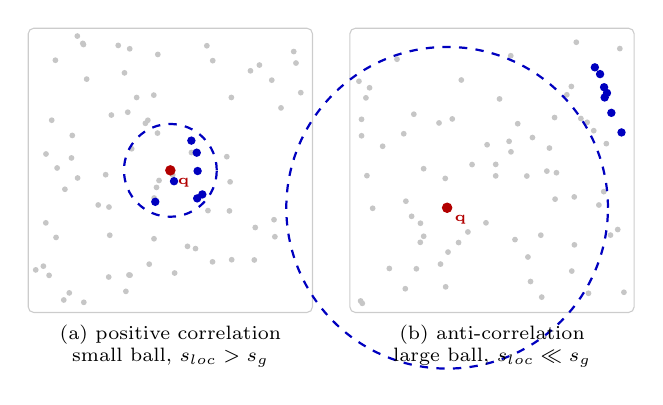
\begin{tikzpicture}[scale=0.95]
\pgfmathsetseed{7}
\begin{scope}
\draw[gray!40, rounded corners=2pt] (-1.9,-1.9) rectangle (1.9,1.9);
\foreach \i in {1,...,70} {\fill[gray!45] ({3.6*rnd-1.8},{3.6*rnd-1.8}) circle (1.1pt);}
\foreach \i in {1,...,7} {\fill[blue!75!black] ({0.9*rnd-0.45},{0.9*rnd-0.45}) circle (1.6pt);}
\fill[red!70!black] (0,0) circle (2pt) node[below right=-1pt, font=\tiny] {$\mathbf{q}$};
\draw[blue!75!black, dashed, thick] (0,0) circle (0.62);
\node[font=\scriptsize, align=center] at (0,-2.35) {(a) positive correlation\\ small ball, $s_{\text{loc}}>s_g$};
\end{scope}
\begin{scope}[xshift=4.3cm]
\pgfmathsetseed{11}
\draw[gray!40, rounded corners=2pt] (-1.9,-1.9) rectangle (1.9,1.9);
\foreach \i in {1,...,70} {\fill[gray!45] ({3.6*rnd-1.8},{3.6*rnd-1.8}) circle (1.1pt);}
\foreach \i in {1,...,7} {\fill[blue!75!black] ({1.2+0.6*rnd},{0.5+1.2*rnd}) circle (1.6pt);}
\fill[red!70!black] (-0.6,-0.5) circle (2pt) node[below right=-1pt, font=\tiny] {$\mathbf{q}$};
\draw[blue!75!black, dashed, thick] (-0.6,-0.5) circle (2.15);
\node[font=\scriptsize, align=center] at (0,-2.35) {(b) anti-correlation\\ large ball, $s_{\text{loc}}\ll s_g$};
\end{scope}
\end{tikzpicture}
\caption{Schematic of local selectivity (illustration, not data). Gray: tuples that fail the filter; blue: matches; red: the query. The dashed ball is the smallest ball around $\mathbf{q}$ that contains $k$ matches, and $h_k$ is the number of tuples inside it. Both panels have the same global selectivity. A post-filter must pass every tuple in the ball, so its cost follows $h_k=k/s_{\text{loc}}$, not $s_g$.}
\label{fig:schematic}
\end{figure}

\emph{It is not just the example.} Among the $\CtxN$ ARXIV-384 test queries whose global selectivity is within $15\%$ of the example's, local selectivity ranges from $\CtxSlocMin\%$ to $\CtxSlocMax\%$, and the fastest correct plan is filter first for $\CtxPre\%$ of them, search first for $\CtxPost\%$ and filter while searching for $\CtxFused\%$. Any rule that picks a plan from the global selectivity alone must treat all of them the same way.

\emph{Where each plan wins.} Writing the plan costs of Section~\ref{sec:costs} as functions of $\sg$ and $\sloc$ shows that filtering first is cheapest only below a boundary $\sg^*(\sloc)$. Because checking the filter column by column already costs time proportional to the table size, a graph plan wins for every $\sg$ once $\sloc$ exceeds roughly $1$--$2\%$, so the boundary is nearly flat and the global selectivity says little about the right plan. The extended version~\cite{hvoextended} states and proves this as a theorem and plots the boundary.

\section{HyperVector-Optimizer}\label{sec:method}
We now describe how HVO makes the decision of Figure~\ref{fig:example} automatically, in a small fraction of the query's running time.

\subsection{Overview}\label{sec:overview}
Before a query runs, HVO answers one question: \emph{how far must the search go to find $k$ matches?} If the answer is ``not far'', searching first is fast; if it is ``very far'', filtering first is usually better. HVO answers the question in four steps, shown in Figure~\ref{fig:arch}.

\noindent\textbf{Step 1: Read the filter.} HVO turns the query's filter into a simple form that it can check quickly. For Query~B, ``published physics papers'' becomes \texttt{published = yes} and \texttt{archive} is one of nine values.

\noindent\textbf{Step 2: Estimate how far the search must go.} HVO keeps a small summary of the data, the \emph{Polytope-Ball Sketch} (HPBS, Section~\ref{sec:sketch}). The summary splits the table into about a thousand groups of similar rows and remembers, for each group, how spread out its vectors are and how many of its rows have each attribute value. From it, HVO estimates the local selectivity without touching the index or the table. For Query~B it estimates $\ExBEstCal\%$ (true value $\ExBSloc\%$); for Query~A, $\ExAEstCal\%$ (true value $\ExASloc\%$).

\noindent\textbf{Step 3: Predict each plan's time.} HVO predicts how long each plan would take (Section~\ref{sec:costs}). The predictions come from timing the plans on the actual machine, not from counting operations. For Query~B, it predicts about $\ExBCostTruePost$\,ms for searching first and $\ExBCostTruePre$\,ms for filtering first.

\noindent\textbf{Step 4: Choose a plan that is safe even if the estimate is wrong.} An estimate can be off by a factor of two or three, so HVO considers a range of possible values instead of a single number, and picks the plan whose \emph{worst case} within that range is fastest (Section~\ref{sec:route}). For Query~B, even in the worst case searching first is predicted to take $\ExBCostLoPost$\,ms, much less than filtering first ($\ExBCostLoPre$\,ms), so HVO searches first. For Query~A, searching first could take up to $\ExACostLoPost$\,ms in the worst case, while filtering first takes about $\ExACostLoPre$\,ms whatever the truth, so HVO filters first.

The chosen plan then runs. Planning reads only the summary, never the index or the data. The summary, the time predictions and the size of the safety range are prepared in advance from training queries, and the same planning code runs in our benchmark and inside PostgreSQL (Section~\ref{sec:pg}).

\begin{figure*}[!t]
\centering
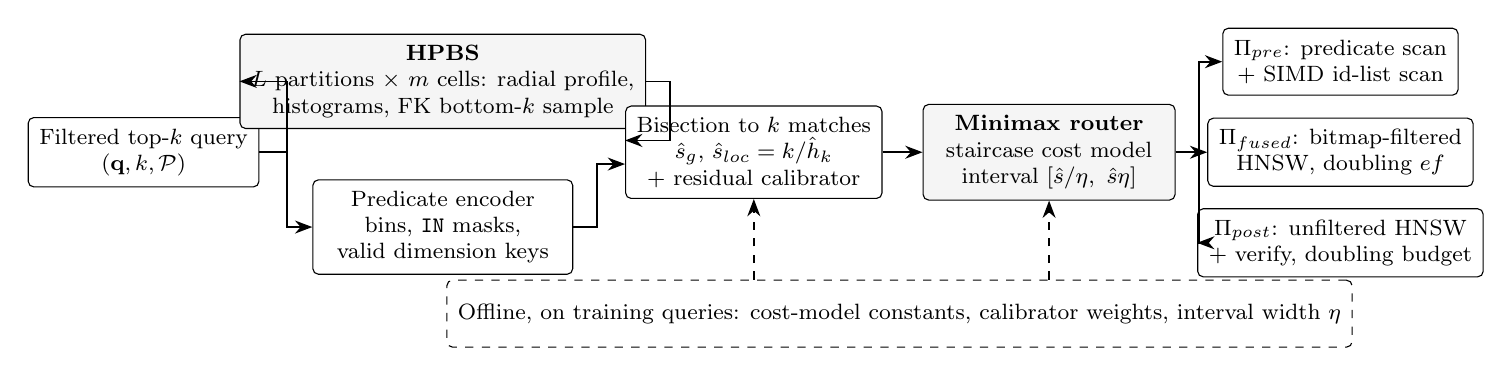
\begin{tikzpicture}[
  font=\footnotesize,
  box/.style={draw, rounded corners=2pt, align=center, minimum height=0.85cm, inner sep=4pt, fill=white},
  graybox/.style={draw, rounded corners=2pt, align=center, minimum height=0.85cm, inner sep=4pt, fill=gray!8},
  dashedbox/.style={draw, dashed, rounded corners=2pt, align=center, minimum height=0.85cm, inner sep=4pt, fill=white},
  arr/.style={-{Stealth[length=2.2mm]}, semithick},
  darr/.style={-{Stealth[length=2.2mm]}, dashed, semithick}
]
\node[box, minimum width=2.2cm] (query) at (0.1, 0.4) {Filtered top-$k$ query\\$(\mathbf{q}, k, \mathcal{P})$};
\node[graybox, minimum width=3.3cm] (sketch) at (3.9, 1.3) {\textbf{HPBS}\\$L$ partitions $\times$ $m$ cells: radial profile,\\histograms, FK bottom-$k$ sample};
\node[box, minimum width=3.3cm] (rel) at (3.9, -0.55) {Predicate encoder\\bins, \texttt{IN} masks,\\valid dimension keys};
\node[box, minimum width=2.9cm] (cal) at (7.85, 0.4) {Bisection to $k$ matches\\$\hat s_g$, $\hat s_{\text{loc}}=k/\hat h_k$\\+ residual calibrator};
\node[graybox, minimum width=3.2cm] (cost) at (11.6, 0.4) {\textbf{Minimax router}\\staircase cost model\\interval $[\hat s/\eta,\ \hat s\eta]$};
\node[box, minimum width=2.6cm] (pre) at (15.3, 1.55) {$\Ppre$: predicate scan\\+ SIMD id-list scan};
\node[box, minimum width=2.6cm] (fused) at (15.3, 0.4) {$\Pfus$: bitmap-filtered\\HNSW, doubling $ef$};
\node[box, minimum width=2.6cm] (post) at (15.3, -0.75) {$\Ppost$: unfiltered HNSW\\+ verify, doubling budget};
\node[dashedbox, minimum width=7.5cm] (calib) at (9.7, -1.65) {Offline, on training queries: cost-model constants, calibrator weights, interval width $\eta$};
\draw[arr] (query.east) -- ++(0.35,0) |- (sketch.west);
\draw[arr] (query.east) -- ++(0.35,0) |- (rel.west);
\draw[arr] (sketch.east) -- ++(0.3,0) |- ([yshift=0.15cm]cal.west);
\draw[arr] (rel.east) -- ++(0.3,0) |- ([yshift=-0.15cm]cal.west);
\draw[arr] (cal.east) -- (cost.west);
\draw[arr] (cost.east) -- ++(0.3,0) |- (pre.west);
\draw[arr] (cost.east) -- (fused.west);
\draw[arr] (cost.east) -- ++(0.3,0) |- (post.west);
\draw[darr] (calib.north -| cost.south) -- (cost.south);
\draw[darr] (calib.north -| cal.south) -- (cal.south);
\end{tikzpicture}
\caption{Architecture of HVO. Planning reads only the sketch, never the vector index. The router evaluates a calibrated cost model at both ends of the estimator's uncertainty interval and runs the plan with the smallest worst-case cost.}
\label{fig:arch}
\end{figure*}

\subsection{Estimating How Far the Search Must Go}\label{sec:sketch}
HPBS answers one question for each query: \emph{how many rows must the search look at before it finds $k$ that pass the filter?} If we list all rows from most to least similar to the query, the answer is how far down the list the $k$-th matching row appears: $h_k$, with local selectivity $k/h_k$ (Definition~\ref{def:sloc}). For Query~B, $h_k=\ExBHk$; for Query~A, $h_k=\ExAHk$. HPBS must answer quickly, without running the search and without touching the index or the table, so it works from a small summary of the data prepared in advance.

\emph{The idea.} HPBS keeps a coarse map of the data. It splits all vectors into $m=1024$ groups (\emph{cells}) of similar items with $k$-means clustering, and remembers three things about every cell $b$:
\begin{itemize}
  \item \emph{Where the cell is and how spread out it is:} its center $\mathbf{c}_b$, its size $N_b$, and 16 quantiles $\rho_{b,1},\ldots,\rho_{b,16}$ of its members' squared distances to the center.
  \item \emph{What its members look like:} for each attribute, the share of members with each value or in each range (for example, $40\%$ physics, $15\%$ from 2010--2015).
  \item \emph{Which linked rows its members point to:} up to $k_{\text{kmv}}=64$ foreign keys, chosen by hashing, with the number of members that carry each one ($\mathcal{K}_b$).
\end{itemize}

\emph{Estimating for a query.} HPBS asks every cell two questions. First, \emph{how many of your members lie within distance $r$ of the query?} With $\delta_b=\|\mathbf{q}-\mathbf{c}_b\|^2$, and because in high dimensions a member's offset from its center is nearly at a right angle to $\mathbf{q}-\mathbf{c}_b$ (so $\|\mathbf{q}-\mathbf{x}\|^2\approx\delta_b+\|\mathbf{x}-\mathbf{c}_b\|^2$), the answer is
\begin{equation}\label{eq:ballcount}
\hat n_b(r) = \frac{N_b}{16}\,\big|\{j : \delta_b + \rho_{b,j} \le r\}\big|.
\end{equation}
Second, \emph{what share of them pass the filter?} HPBS reads each condition's share $\hat\sigma^{(j)}_b$ from the stored statistics. For a condition on the linked table, it evaluates the condition on that small table to get the set $\mathcal{V}$ of valid keys, and estimates the share of the cell's rows that point to a valid key as
\begin{equation}\label{eq:kmv_join}
\hat\sigma^{\text{join}}_b = \frac{\sum_{h\in\mathcal{K}_b} f_b(h)\,\mathbb{I}[h\in\mathcal{V}]}{\sum_{h\in\mathcal{K}_b} f_b(h)},
\end{equation}
where $f_b(h)$ is the number of the cell's rows with key $h$. Assuming the conditions are independent \emph{within} a cell, the cell's matching share is $\hat\sigma_b=\prod_j\hat\sigma^{(j)}_b\cdot\hat\sigma^{\text{join}}_b$. Multiplying the two answers and adding over all cells gives the expected number of matches within distance $r$, $\hat M(r)=\sum_b\hat n_b(r)\hat\sigma_b$. HPBS finds the distance $\hat r$ at which $\hat M(\hat r)=k$ by repeatedly halving the search range (26 steps), and returns
\begin{equation}\label{eq:sloc_hat}
\hat s_{\text{loc}} = \min\!\Big(1,\ \frac{k}{\sum_b \hat n_b(\hat r)}\Big), \qquad \hat s_g = \frac{1}{N}\sum_b N_b\hat\sigma_b .
\end{equation}
Algorithm~1 lists the steps.

\begin{table}[!t]
\footnotesize
\centering
\caption{Algorithm 1: HPBS query-time estimation (one partition; the sketch returns the median over $L$).}
\label{alg:hpbs}
\begin{tabular}{p{0.95\columnwidth}}
\toprule
\textbf{Input:} $\mathbf{q}$, $k$, predicate $\mathcal{P}$, partition $\{\mathbf{c}_b, N_b, \rho_{b,\cdot}, \text{hist}_b, \mathcal{K}_b\}_{b=1}^m$.\\
1: Encode $\mathcal{P}$: boundary bins and offsets of each range, bitmask of each \texttt{IN} list, valid key set $\mathcal{V}$ of the dimension predicate.\\
2: $\boldsymbol{\delta}\leftarrow \|\mathbf{c}\|^2 - 2\,\mathbf{C}\mathbf{q} + 1$ \hfill $\triangleright$ one \texttt{sgemv}\\
3: \textbf{for} each cell $b$: $\hat\sigma_b\leftarrow\prod_j\hat\sigma_b^{(j)}\cdot\hat\sigma_b^{\text{join}}$ (Eq.~\eqref{eq:kmv_join}); $\hat s_g \mathrel{+}= N_b\hat\sigma_b/N$.\\
4: $\mathcal{C}\leftarrow\{b:\hat\sigma_b>0\}$; $lo\leftarrow0$; $hi\leftarrow\max_{b\in\mathcal{C}}\delta_b+\rho_{b,16}$.\\
5: \textbf{repeat} 26 times: $r\leftarrow(lo+hi)/2$; \textbf{if} $\sum_{b\in\mathcal{C}}\hat n_b(r)\hat\sigma_b<k$ \textbf{then} $lo\leftarrow r$ \textbf{else} $hi\leftarrow r$; $\mathcal{C}\leftarrow\{b\in\mathcal{C}:\delta_b\le hi\}$.\\
6: \textbf{return} $\hat s_g$, $\hat s_{\text{loc}}\leftarrow\min(1, k/\sum_b\hat n_b(hi))$.\\
\bottomrule
\end{tabular}
\end{table}

\emph{Why this captures correlation.} HPBS assumes independence only \emph{inside} a cell. Across cells it keeps the real picture: physics papers are common in some cells and absent from others. This is exactly the information that is lost when an optimizer counts matches over the whole table.

\emph{Combining and correcting.} HPBS builds $L=4$ such maps with different random starts and returns the median of their four estimates, which smooths out unlucky groupings. A small neural network with $\CalParamsA$ parameters, trained only on the training queries, then corrects the remaining bias: $\hat s_{\text{loc}}\leftarrow\operatorname{clip}(\hat s^{\text{raw}}_{\text{loc}}e^{f_\Theta(\mathbf{z})},k/N,1)$, where $\mathbf{z}$ holds twelve features of the raw estimate and the query~\cite{hvoextended}. It mainly helps when a query lies very close to a cell's center, or when the independence assumption inside a cell is poor. The correction takes about $\CalUsA\,\mu$s and mostly removes large errors: on ARXIV-384 the 99th-percentile Q-error falls from $\QHpbsPnnC$ to $\QHpbsPlusCalPnnC$.

\emph{Example.} For Query~A, the filter selects physics papers, but the cells around this computer-science paper contain almost none, so the estimated distance must grow until it reaches cells where physics papers are common. HPBS estimates a local selectivity of $\ExAEstCal\%$, close to the true $\ExASloc\%$. For comparison, looking at the index's 256 nearest neighbors finds \emph{no} physics paper at all, so that method can only report ``less than $\ExAEstProbe\%$'' (Section~\ref{sec:eval_card}). For Query~B, the cells near the query contain many published physics papers, and HPBS estimates $\ExBEstCal\%$ (true value $\ExBSloc\%$). Both estimates are within a factor of $2.5$ of the truth, which is enough for HVO to pick the right plan.

\emph{Where the errors come from.} Let $n_b(r)$ and $M_b(r)$ be the true numbers of rows and of matches of cell $b$ within squared distance $r$, $\sigma_b(r)=M_b(r)/n_b(r)$, and $h(j)$ the number of rows within the distance of the $j$-th closest match, so $h_k=h(k)$. Proposition~\ref{prop:decomp} splits the estimation error into two parts: errors in \emph{how many} rows of each cell lie within a given distance ($\alpha$), and errors in \emph{what share} of them pass the filter ($\beta$).
\begin{proposition}[Deterministic error decomposition]\label{prop:decomp}
Suppose that for every $r$ and $b$ the geometric and cell estimates satisfy
\[
\hat n_b(r)\in\big[n_b(r)/\alpha,\ \alpha n_b(r)\big],\qquad \hat\sigma_b\in\big[\sigma_b(r)/\beta,\ \beta\sigma_b(r)\big].
\]
Then
\[
\text{Q-error}(\hat s_{\text{loc}}, \sloc) \le \alpha\cdot\psi(\alpha\beta), \quad \psi(t)=\max\Big(\frac{h(\lceil tk\rceil)}{h(k)},\ \frac{h(k)}{h(\lfloor k/t\rfloor)}\Big).
\]
If matches are locally uniform around $\mathbf{q}$ ($h(j)\propto j$), then $\psi(t)\approx t$ and the Q-error is at most $\alpha^2\beta$.
\end{proposition}
Smaller cells reduce $\alpha$, and finer statistics reduce part of $\beta$. The rest of $\beta$ comes from relationships \emph{inside} a cell, which a summary of this kind cannot see. That is why HPBS is less accurate on AMAZON-384, where each filter is built from the query product itself and matches cluster tightly around the query (Section~\ref{sec:eval_card}). The proposition explains where errors come from; it does not promise an error bound for every dataset, and we prove nothing about the calibrator. The proof is in the extended version~\cite{hvoextended}.

\emph{Size and cost.} For one million vectors, HPBS takes $\QHpbsMBA$, $\QHpbsMBC$ and $\QHpbsMBB$\,MiB for 128-, 384- and 768-dimensional vectors ($\SketchPctB$--$\SketchPctA\%$ of the size of the vectors themselves). It is built in $\BuildHpbsA$--$\BuildHpbsB$\,s, against $\BuildHnswA$--$\BuildHnswB$\,s for the HNSW index on 10 threads. Adding a row updates one cell in each map; we have not evaluated workloads with frequent updates.

\subsection{The Three Plans}\label{sec:plans}
All plans run on one thread. \emph{Filter first} ($\Ppre$) checks the filter column by column and compares the query with each matching row in a C loop (NEON SIMD). \emph{Search first} ($\Ppost$) is a \emph{resumable} scan over a faiss~\cite{douze2024faiss} HNSW graph ($M=32$, $ef_{\text{construction}}=200$) in the spirit of \texttt{pgvector}'s iterative scan: it returns rows in batches of $k, k, 2k, 4k, \ldots$ in roughly decreasing similarity, checks each batch against the filter, and continues from where it stopped until $k$ rows have passed (at most $2^{17}$). \emph{Filter while searching} ($\Pfus$) is ACORN-1~\cite{patel2024acorn} ($M=32$, $M_\beta=64$), which doubles its search budget from 64 until it has $k$ results and a doubled budget returns the same set. Running ACORN at one million vectors required fixing two memory bugs in its reference code; the fix has been submitted upstream. Because each plan keeps going until it has its answer, its running time does not depend on the optimizer's estimate.

\subsection{Predicting Plan Costs from Measurements}\label{sec:costs}\label{sec:routing}
A cost model answers the question: \emph{if the local selectivity were $s$, how long would each plan take?} A common shortcut is to count operations, such as distance computations. We instead fit each plan's cost to running times measured on the target machine, because the same number of distance computations costs very different amounts in a sequential scan and in a random walk over a graph (Section~\ref{sec:eval_hw} shows that counting makes the routing 1.6--6.3$\times$ slower).

\emph{Graph plans grow in rounds.} A graph plan doubles its budget in each round ($e_i=e_0 2^i$) and stops once the budget reaches what the query needs, $\nu$. It therefore runs $j(\nu)=\lceil\log_2(\nu/e_0)\rceil^+$ rounds, capped at the budget limit. If a round with budget $e$ costs $b_0+b_1e^\gamma$, the plan's cost is a ``staircase'' in $\nu$:
\begin{equation}\label{eq:stair}
\operatorname{St}(\nu;b_0,b_1,\gamma)=\sum_{i=0}^{j(\nu)}\big(b_0+b_1(e_02^i)^\gamma\big).
\end{equation}
\emph{The three costs.} Let $C_{\text{rel}}=c_0+c_1N|\mathcal{P}|+c_2N\,\mathbb{I}[\text{join}]$ be the cost of checking the filter over all rows. Then
\begin{align}
C(\Ppre)&=C_{\text{rel}}+a_0+c_{\text{scan}}\,\sg N,\label{eq:cost_pre}\\
C(\Ppost)&=\operatorname{St}\!\big(k/\sloc;\,\theta_{\text{post}}\big),\label{eq:cost_post}\\
C(\Pfus)&=C_{\text{rel}}+\operatorname{St}^{+1}\!\big(c_f(k/\sloc)^{\beta_f};\,\theta_{\text{fused}}\big),\label{eq:cost_fused}
\end{align}
where $\operatorname{St}^{+1}$ adds ACORN's final confirmation round. In words: filtering first pays for checking the filter plus one comparison per matching row; searching first needs exactly $h_k=k/\sloc$ rows (Definition~\ref{def:sloc}); and filtering while searching pays for checking the filter plus a graph walk whose budget grows faster than $h_k$, which the exponent $\beta_f$ captures.

\emph{Fitting the constants.} All constants are fitted on the training queries from their \emph{true} selectivities and measured times, the linear ones by non-negative least squares and the staircase ones by nonlinear least squares in log space ($\gamma\in[0.3,2.5]$). Exponents above one are common, because a graph search's priority queues make large budgets disproportionately expensive. ACORN's cost could not be fitted by a smooth staircase, so we model it with a monotone (isotonic) curve in $h_k$.

\emph{Example.} At the true selectivities, the model predicts $\ExACostTruePre$\,ms (filter first), $\ExACostTrueFused$\,ms (filter while searching) and $\ExACostTruePost$\,ms (search first) for Query~A, against measured times of $\ExATPre$, $\ExATFused$ and $\ExATPost$\,ms; and $\ExBCostTruePre$, $\ExBCostTrueFused$ and $\ExBCostTruePost$\,ms for Query~B, against $\ExBTPre$, $\ExBTFused$ and $\ExBTPost$\,ms. The model picks the oracle's plan for both queries. It overestimates ACORN on Query~A, where ACORN is in fact fast but returns only $\ExARecFused$ of the correct answers; ACORN's cost is the hardest to model (Section~\ref{sec:eval_e2e}).

\subsection{Choosing a Plan Robustly}\label{sec:route}
An estimate can be off by a factor of two or three, and the damage of a wrong estimate is lopsided. Filtering first costs the same whatever the local selectivity, while a graph plan's cost explodes when the local selectivity is lower than believed. HVO therefore asks, for each plan, \emph{``how slow could this plan be if the truth were anywhere in my uncertainty range?''}, and picks the plan whose worst case is fastest.

\emph{Point and minimax routing.} \emph{Point routing} trusts the estimate and picks $\arg\min_\Pi C(\Pi;\hat s_g,\hat s_{\text{loc}})$. \emph{Minimax routing} considers the range $I=[\hat s_{\text{loc}}/\eta,\ \hat s_{\text{loc}}\eta]$ and picks
\begin{equation}\label{eq:robust}
\begin{aligned}
\hat\Pi&=\arg\min_\Pi\ \max_{s\in I}C(\Pi;\hat s_g,s)\\
&=\arg\min_\Pi\ \max\big(C(\Pi;\hat s_g,\hat s_{\text{loc}}/\eta),\ C(\Pi;\hat s_g,\hat s_{\text{loc}}\eta)\big).
\end{aligned}
\end{equation}
The second line holds because every plan's cost only goes up as $\sloc$ goes down, so the worst case is at one end of the range. We set $\eta$ to the value that covers $90\%$ of the estimator's errors on the training queries, fixed before looking at test data ($\eta=\EtaHvoA$ and $\EtaHvoB$ on the synthetic datasets). Because the cost of filtering first does not depend on $\sloc$, minimax routing prefers it whenever the estimate is uncertain.

\emph{Example.} On ARXIV-384, $\eta=\ExEta$, so Query~B's range is $[\ExBEstLo\%,\ \ExBEstHi\%]$. Even at the bad end of that range, searching first is predicted to take $\ExBCostLoPost$\,ms, against $\ExBCostLoPre$\,ms for filtering first, so HVO searches first. Query~A's range is $[\ExAEstLo\%,\ \ExAEstHi\%]$. At its bad end, searching first could take $\ExACostLoPost$\,ms and filtering while searching $\ExACostLoFused$\,ms, while filtering first takes $\ExACostLoPre$\,ms whatever the truth, so HVO filters first. Both are the oracle's choices.

\emph{Recall-aware routing.} Graph plans can miss correct answers. For each graph plan we fit a small logistic model, on the training queries, that predicts the chance of getting at least $9$ of the top $10$ from values known at planning time (the two estimates, the number of filter conditions and whether there is a join). The recall-aware router allows a graph plan only if this chance is at least $0.9$, and otherwise filters first. This trades speed for completeness, and we report both variants.

\emph{Native planner.} The whole decision---sketch estimate, calibrator, recall check and minimax costing---runs in one C function, \texttt{hvo\_plan}, shared by the benchmark and the PostgreSQL extension. It takes the encoded filter and the query vector and returns the plan.

\subsection{Guarantees}\label{sec:theory}
The example shows minimax routing making the right choice on two queries. The results below say when it is guaranteed to, and how much an estimation error of a given size can cost. Three facts drive them. A graph plan doubles its budget in rounds, so a small estimation error changes its cost by at most a few rounds (Lemma~\ref{lem:sens}). Filtering first costs the same whatever the local selectivity, so a minimax router never gives up a query whose best plan is filtering first (Theorem~\ref{thm:robust}). And a rule that sees only the share of matching rows cannot tell the two panels of Figure~\ref{fig:schematic} apart, so it can be made arbitrarily slow (Proposition~\ref{prop:unbounded}).

We measure the cost of a wrong choice by the \emph{regret} $\mathcal{R}=C(\hat\Pi;s)/C(\Pi^*;s)$: the cost of the chosen plan divided by the cost of the best plan $\Pi^*$ at the true selectivities $s=(\sg,\sloc)$. A regret of 1 means the best plan was chosen. The results concern the cost model of Section~\ref{sec:costs}; measured regret also includes the model's own error, which we report in Section~\ref{sec:eval}. All statements hold query by query; proofs are in the extended version~\cite{hvoextended}.
\begin{lemma}[Sensitivity of staircase plans]\label{lem:sens}
Let a plan's cost be $A+\operatorname{St}(c\,(k/s)^\beta;b_0,b_1,\gamma)$ with $A,b_0,b_1\ge0$ and $\gamma>0$. If $\hat s/s\in[1/\eta,\eta]$, then its cost at $\hat s$ is within a factor $\Lambda_{\beta,\gamma}(\eta)$ of its cost at $s$, where
\[
\Lambda_{\beta,\gamma}(\eta)=1+\delta\,2^{\gamma\delta},\qquad \delta=\lceil\beta\log_2\eta\rceil .
\]
\end{lemma}

Let $\Lambda=\max(\eta_g,\Lambda_{1,\gamma_{\text{post}}}(\eta),\Lambda_{\beta_f,\gamma_{\text{fused}}}(\eta))$, where $\eta_g$ bounds the multiplicative error of $\hat s_g$, which enters $C(\Ppre)$ affinely.

\begin{theorem}[Point routing]\label{thm:regret}
If $\hat s_g/\sg\in[1/\eta_g,\eta_g]$ and also $\hat s_{\text{loc}}/\sloc\in[1/\eta,\eta]$, then point routing has $\mathcal{R}\le\Lambda^2$. If, in addition, $\hat s_g=\sg$ and either $\hat\Pi$ or $\Pi^*$ is $\Ppre$, then $\mathcal{R}\le\Lambda$.
\end{theorem}

\begin{theorem}[Minimax routing]\label{thm:robust}
Suppose $\hat s_g=\sg$ and $\sloc\in I=[\hat s_{\text{loc}}/\eta,\hat s_{\text{loc}}\eta]$. Then minimax routing (Eq.~\eqref{eq:robust}) satisfies: (i) if $\Pi^*=\Ppre$, then $\mathcal{R}=1$; (ii) in all cases $\mathcal{R}\le\Lambda(\eta^2)$.
\end{theorem}

\begin{proposition}[Global-selectivity routing]\label{prop:unbounded}
Let a router choose its plan as any function of $\sg$ alone. Let graph-plan costs satisfy $C_G(1)\le C_1$ and $C_G(k/N)\ge bN^\gamma$ for constants $C_1,b,\gamma>0$, and let $C(\Ppre)=a+c'\sg N$, which holds when predicates are evaluated through an index at a cost proportional to their output. Then for $N$ large enough that $k\le\sqrt{bN^\gamma C_1/c'}$, its worst-case regret over instances with that $N$ is at least $\sqrt{bN^\gamma/(c'C_1)}\,/\,(1+o(1))$, that is, $\Omega(N^{\gamma/2})$.
\end{proposition}

\subsection{Integration into PostgreSQL}\label{sec:pg}
We implemented HVO as a PostgreSQL~16 extension (\texttt{hvo\_pg}) for \texttt{pgvector}~0.8.7, using PostgreSQL's \texttt{planner\_hook}, which lets an extension see every query before it is planned. For a query that orders by \texttt{embedding <\#> $\mathbf{q}$} with a \texttt{LIMIT}, the hook does three things:
\begin{itemize}
    \item It reads the query vector, $k$, and the filter: ranges, equalities and \texttt{IN} lists on the main table, and conditions on the linked table written as \texttt{fk IN (SELECT id FROM dims WHERE \ldots)}.
    \item It encodes the filter for the summary, evaluating conditions on the linked table against an in-memory copy of that small table.
    \item It calls \texttt{hvo\_plan} and steers PostgreSQL's own planner toward the chosen plan with standard settings, as the \texttt{pg\_hint\_plan} extension does: it turns index scans off to filter first, and turns sequential and bitmap scans off to use \texttt{pgvector}'s iterative HNSW scan.
\end{itemize}
\texttt{pgvector} cannot filter while searching, so in PostgreSQL the choice is between two plans. The model file holds the summary, the calibrator, the uncertainty range, and cost and recall models fitted to PostgreSQL's own running times and recall on the training queries. The hook is about 660 lines of C plus the shared planner code.

\emph{Example.} Query~B reaches PostgreSQL as
\begin{center}
\footnotesize
\begin{tabular}{@{}l@{}}
\texttt{SELECT id FROM items WHERE published IN (1)}\\
\texttt{\ \ AND archive IN (4,6,9,14,21,22,27,28,30)}\\
\texttt{\ \ ORDER BY embedding <\#> '[$\ldots$]' LIMIT 10}
\end{tabular}
\end{center}
where the literal holds the 384 numbers of the query paper's embedding. The hook reads the vector, the two conditions and the limit, receives ``search first'' from the planner, and lets PostgreSQL plan with sequential and bitmap scans turned off, so \texttt{pgvector}'s iterative HNSW scan is used. For Query~A it receives ``filter first'' and turns index scans off, so PostgreSQL filters the table and sorts the matches by distance. Queries the hook does not recognize are planned normally.

\section{Evaluation}\label{sec:eval}
We ask four questions. How accurate and fast is HPBS compared with histograms, exact counts, sampling and index probing (Section~\ref{sec:eval_card})? Does better estimation lead to faster queries (Section~\ref{sec:eval_e2e})? How much do the compare loop and each part of HVO matter (Section~\ref{sec:eval_hw})? And how does the cost of wrong choices compare with the proven bounds (Section~\ref{sec:eval_hw})? Every plan runs for every test query on real hardware, so the best plan is measured, not modeled. Section~\ref{sec:discussion} discusses limitations.

\subsection{Evaluation Settings}\label{sec:setup}
\emph{Hardware and software.} Apple M4 (16\,GB), macOS~26.3, Python~3.14 with NumPy~2.4, scikit-learn~1.8 and faiss-cpu~1.13.2, C code compiled with clang~17 (\texttt{-O3}), PostgreSQL~16.14 with \texttt{pgvector}~0.8.7. Every latency is measured on one thread; each plan runs once as a warm-up and twice timed, and we report the slower run. PostgreSQL uses \texttt{shared\_buffers}=4\,GB, no parallel query or JIT, and \texttt{pgvector}'s default HNSW parameters; its latencies are client wall-clock times, including planning.

\emph{Datasets.} \textbf{ARXIV-384}: one million papers from the CC0 arXiv-abstracts-2021 dump~\cite{arxivdump}, embedded with all-MiniLM-L6-v2~\cite{reimers2019sbert} (384 dimensions, title and abstract), with real attributes (archive, published, year, numbers of categories, authors and abstract words) and a foreign key to its 172 primary categories. \textbf{AMAZON-384}: $990{,}000$ products from Amazon Reviews 2023~\cite{hou2024amazon} in four departments, embedded the same way, with real attributes (department, categories, price, rating, number of ratings, features, description length) and a foreign key to about $144{,}000$ stores. Its filters are built from the query product, as a shopper would filter (same or another department, a price band, a minimum rating, a seller tier). \textbf{SYN-128} and \textbf{SYN-768}: one million synthetic vectors from a topic mixture, with attributes generated from the topics at graded strength. Query vectors are held-out items (real data) or noisy data vectors (synthetic). Both real benchmarks are public with exact answers~\cite{hvobench}.

\emph{Workloads.} Filters combine 1--3 conditions: ranges, \texttt{IN} lists and conditions on the linked table. On SYN-128, SYN-768 and ARXIV-384 they are drawn independently of the query, so filter and query are related only through the data itself. Each benchmark has $1000$ training and $1500$ test queries (queries with no match are dropped); the test splits contain $\nAntiC/\nIndepC/\nPosC$ (ARXIV-384) and $\nAntiD/\nIndepD/\nPosD$ (AMAZON-384) anti-correlated/independent/positively correlated queries. We use $k=10$ unless stated. Everything fitted uses only the training split.

\emph{Baselines.} Estimators: PostgreSQL-style 1-D histograms with independence; the exact global count (Milvus-style); a $1\%$ sample; and an Exqutor-style HNSW probe of the 256 nearest neighbors. Each feeds the same cost model. Routers also include the three single plans and the best global-selectivity rules (two- and three-way thresholds tuned on the training split). Inside PostgreSQL we compare \texttt{pgvector} with default settings, \texttt{pgvector}'s iterative scan (\texttt{strict\_order}), Exqutor~\cite{exqutor2026} built from its released code, both forced plans, and the HVO hook with and without the recall constraint. Exqutor's estimator only activates for vector \emph{range} predicates over more than two tables, so on these queries it plans like \texttt{pgvector}~0.7.1.

\emph{Metrics and statistics.} The oracle runs every plan and takes the fastest with Recall@$k\ge0.9$; other routers are charged their plan's latency plus their planning time. Regret is a router's latency divided by the oracle's. For differences between routers we report paired 95\% percentile-bootstrap intervals over test queries (2000 resamples); they capture variation across queries in one run per setting, not repeated-run timing noise.

\subsection{Estimation Accuracy}\label{sec:eval_card}
Table~\ref{tab:cardinality} and Figure~\ref{fig:card} report how far each estimate is from the truth, measured as the Q-error (the larger of estimate/truth and truth/estimate; 1 is perfect).

\emph{Estimators that ignore the vectors fail when filters and similarity are related, worst on real data.} Histograms and exact counts both assume that the share of matches near the query equals the share in the whole table. Their 99th-percentile errors reach $\QPgHistPnnC$ and $\QExactAviPnnC$ on ARXIV-384 and $\QPgHistPnnD$ and $\QExactAviPnnD$ on AMAZON-384, against $\QPgHistPnnA$ and $\QExactAviPnnA$ on SYN-128. The errors concentrate where matches lie far from the query and where they are rare. Knowing the global share exactly does not help, because the mistake is in assuming that the local share equals it; the exact count also costs $\QExactAviUsC\,\mu$s of planning time.

\emph{Sampling sees too little.} A $1\%$ sample (99th-percentile error $\QSampleOnePnnC$ and $\QSampleOnePnnD$ on the real data) contains very few matches near the query.

\emph{Probing the index works where matches are dense and fails where they are rare.} The index probe is the strongest baseline. Its median error is the lowest of all estimators on every dataset (for example $\QProbeMedC$ on ARXIV-384), because it looks at the query's actual neighbors. When none of the first 256 neighbors match, though, it can only say ``fewer than this'', so its 99th-percentile error is $\QProbePnnC$ on ARXIV-384, and $\QProbeRareC$ on queries with rare local matches. It also spends $\QProbeUsC\,\mu$s accessing the index during planning.

\emph{HPBS.} The calibrated sketch has the lowest 99th-percentile error on ARXIV-384 ($\QHpbsPlusCalPnnC$), SYN-128 ($\QHpbsPlusCalPnnA$) and SYN-768 ($\QHpbsPlusCalPnnB$), and a version of HPBS has the lowest error on rare matches on all three ($\QHpbsPlusCalRareC$ against $\QProbeRareC$ for the probe on ARXIV-384). AMAZON-384 is the exception: there the probe is slightly more accurate ($\QProbePnnD$ against $\QHpbsPlusCalPnnD$). Its filters are built from the query product, so matches crowd right around the query; this happens \emph{inside} a cell, where HPBS averages it away and the probe sees it (the $\beta$ term of Proposition~\ref{prop:decomp}). The calibrator mainly removes large errors: the 99th percentile falls from $\QHpbsPnnC$ to $\QHpbsPlusCalPnnC$ on ARXIV-384 and from $\QHpbsPnnD$ to $\QHpbsPlusCalPnnD$ on AMAZON-384. On the real data, a single map ($L=1$) is about as accurate after calibration ($\QHpbsLOnePlusCalPnnC$ and $\QHpbsLOnePlusCalPnnD$) at less than half the planning time; on synthetic data it is less accurate.

\emph{Values shared by many rows.} $57\%$ of Amazon products have price 0; giving such values their own histogram bin (in the sketch and, as a most-common-value list, in the baseline) was necessary for accurate estimates.

\begin{table*}[!t]
\footnotesize
\renewcommand{\arraystretch}{0.95}
\centering
\caption{Local-selectivity Q-error on the test split, by correlation regime and for rare local matches ($\sloc<10^{-3}$), and median planning-time cost of the estimator. Lower is better.}
\label{tab:cardinality}
\setlength{\tabcolsep}{4.2pt}
\begin{tabular}{lccccccccccc}
\toprule
 & \multicolumn{3}{c}{Anti-correlated} & \multicolumn{3}{c}{Independent} & \multicolumn{3}{c}{Positively correlated} & Rare & Time \\
\cmidrule(lr){2-4}\cmidrule(lr){5-7}\cmidrule(lr){8-10}
Estimator & P50 & P95 & P99 & P50 & P95 & P99 & P50 & P95 & P99 & P99 & ($\mu$s) \\
\midrule
\csname @@input\endcsname generated/card_rows.tex
\bottomrule
\end{tabular}
\end{table*}

\begin{figure*}[!t]
\centering
\begin{tikzpicture}
\begin{axis}[
    name=q1, width=0.34\textwidth, height=4.6cm,
    xmode=log, ymode=log, xmin=5e-5, xmax=1, ymin=1, ymax=200,
    xlabel={True local selectivity $s_{\text{loc}}$}, ylabel={P90 Q-error per bin},
    xlabel style={font=\scriptsize}, ylabel style={font=\scriptsize}, ticklabel style={font=\scriptsize},
    title style={font=\footnotesize\bfseries}, title={(a) Q-error vs.\ $s_{\text{loc}}$, SYN-128},
    legend style={at={(0.98,0.98)}, anchor=north east, font=\tiny, draw=none, fill=white, inner sep=1pt},
    grid=major, grid style={dashed, gray!30}]
\addplot[red!75!black, mark=triangle*, thick] coordinates {\binqPgHistA};
\addplot[orange!85!black, mark=square*, thick] coordinates {\binqSampleOneA};
\addplot[teal!80!black, mark=diamond*, thick] coordinates {\binqProbeA};
\addplot[blue!80!black, mark=*, very thick] coordinates {\binqHpbsPlusCalA};
\legend{1-D hist.+AVI, 1\% sample, HNSW probe, HPBS+cal.}
\end{axis}
\begin{axis}[
    name=q2, at={(q1.east)}, anchor=west, xshift=1.2cm, width=0.34\textwidth, height=4.6cm,
    xmode=log, ymode=log, xmin=5e-5, xmax=1, ymin=1, ymax=200,
    xlabel={True local selectivity $s_{\text{loc}}$},
    xlabel style={font=\scriptsize}, ticklabel style={font=\scriptsize},
    title style={font=\footnotesize\bfseries}, title={(b) Q-error vs.\ $s_{\text{loc}}$, ARXIV-384},
    grid=major, grid style={dashed, gray!30}]
\addplot[red!75!black, mark=triangle*, thick] coordinates {\binqPgHistC};
\addplot[orange!85!black, mark=square*, thick] coordinates {\binqSampleOneC};
\addplot[teal!80!black, mark=diamond*, thick] coordinates {\binqProbeC};
\addplot[blue!80!black, mark=*, very thick] coordinates {\binqHpbsPlusCalC};
\end{axis}
\begin{axis}[
    name=q3, at={(q2.east)}, anchor=west, xshift=1.2cm, width=0.34\textwidth, height=4.6cm,
    xmode=log, ymode=log, xmin=5e-5, xmax=1, ymin=0.03,
    xlabel={True local selectivity $s_{\text{loc}}$}, ylabel={Median latency (ms)},
    xlabel style={font=\scriptsize}, ylabel style={font=\scriptsize}, ticklabel style={font=\scriptsize},
    title style={font=\footnotesize\bfseries}, title={(c) Plan latency vs.\ $s_{\text{loc}}$, SYN-128},
    legend style={at={(0.98,0.98)}, anchor=north east, font=\tiny, draw=none, fill=white, inner sep=1pt},
    grid=major, grid style={dashed, gray!30}]
\addplot[blue!75!black, thick, dashed] coordinates {\binpreA};
\addplot[purple!80!black, thick, dashdotted] coordinates {\binfusedA};
\addplot[red!75!black, thick, dotted] coordinates {\binpostA};
\addplot[green!55!black, very thick, mark=*] coordinates {\binhvoA};
\addplot[black, thin, mark=o] coordinates {\binoracleA};
\legend{$\Pi_{\text{pre}}$, $\Pi_{\text{fused}}$, $\Pi_{\text{post}}$, HVO, Oracle}
\end{axis}
\end{tikzpicture}
\caption{(a, b) P90 Q-error within bins of true local selectivity: the baselines degrade as matches become rare near the query, and HPBS does not. (c) Median latency of each plan by true local selectivity on SYN-128, with HVO (including planning time) and the oracle. Pre-filtering is flat in $s_{\text{loc}}$; the graph plans' cost explodes as $s_{\text{loc}}$ falls.}
\label{fig:card}
\end{figure*}

\begin{table*}[!t]
\footnotesize
\renewcommand{\arraystretch}{0.94}
\centering
\caption{End-to-end routing on the real datasets ($k=10$): latency (ms, including planning time), mean Recall@10, share of queries with Recall@10 $<0.9$, plan accuracy against the oracle, measured regret, and median planning time ($\mu$s). CM: the calibrated cost model of Section~\ref{sec:routing}; ``robust'': minimax routing with the interval width fitted on the training split.}
\label{tab:e2e}
\setlength{\tabcolsep}{4.2pt}
\begin{tabular}{lcccccccccc}
\toprule
Router & Mean & P50 & P95 & P99 & Recall & Low (\%) & Acc.\ (\%) & Mean reg. & P99 reg. & Plan ($\mu$s) \\
\midrule
\csname @@input\endcsname generated/e2e_real_rows.tex
\bottomrule
\end{tabular}
\end{table*}

\begin{table*}[!t]
\footnotesize
\renewcommand{\arraystretch}{0.94}
\centering
\caption{Inside PostgreSQL~16 + \texttt{pgvector} on the real datasets ($k=10$, test split): client latency in ms (including planning), mean Recall@10, and share of queries with Recall@10 $<0.9$. The oracle takes the faster forced plan that meets Recall@10 $\ge0.9$ (pre-filtering if neither does). Exqutor was run on ARXIV-384 only; it needs its own patched PostgreSQL build and a separate copy of the data.}
\label{tab:pg}
\setlength{\tabcolsep}{4.4pt}
\begin{tabular}{lcccccccccc}
\toprule
 & \multicolumn{5}{c}{ARXIV-384} & \multicolumn{5}{c}{AMAZON-384} \\
\cmidrule(lr){2-6}\cmidrule(lr){7-11}
Configuration & Mean & P50 & P99 & Recall & Low (\%) & Mean & P50 & P99 & Recall & Low (\%) \\
\midrule
\csname @@input\endcsname generated/pg_rows.tex
\bottomrule
\end{tabular}
\end{table*}

\subsection{End-to-End Latency}\label{sec:eval_e2e}
Table~\ref{tab:e2e} reports latency, recall and regret for every router on the real data at $k=10$ (the synthetic-data table is in the extended version~\cite{hvoextended}). Figure~\ref{fig:cdf} shows the full distribution of query times, and Figure~\ref{fig:card}(c) where the plans cross on SYN-128.

\emph{No single plan works for every query.} Filtering first always pays for checking the whole table (mean $\RAlwaysPreMeanC$\,ms on ARXIV-384). Searching first is the best plan for most queries, but queries with rare local matches push its 99th percentile to $\RAlwaysPostPnnC$\,ms. ACORN-1 is rarely fastest and misses answers when matches are rare near the query (mean recall $\RAlwaysFusedRecA$ when used for every SYN-128 query).

\emph{On real data, HVO cuts the slowest queries, and on ARXIV-384 also the average.} On ARXIV-384, HVO averages $\RHvoMeanC$\,ms against $\RGlobalTwoWayMeanC$\,ms for the best tuned global rule ($\MeanGainVsGlobalC\%$ lower; 95\% interval $\GainLoHvoC$--$\GainHiHvoC\%$), and its 99th-percentile latency is $\RHvoPnnC$\,ms against $\RGlobalTwoWayPnnC$\,ms. On AMAZON-384 the average is $\MeanGainVsGlobalD\%$ lower ($\RHvoMeanD$ vs.\ $\RGlobalTwoWayMeanD$\,ms), but the interval ($\GainLoHvoD$ to $\GainHiHvoD\%$) includes zero, so this gain is not established with our number of queries; the gain on the slowest queries is clear ($\RHvoPnnD$ vs.\ $\RGlobalTwoWayPnnD$\,ms, Figure~\ref{fig:cdf}b). HVO's recall equals the global rule's ($\RHvoRecC$ vs.\ $\RGlobalTwoWayRecC$ on ARXIV-384), and its latency is close to that of the same cost model given the true selectivities ($\RCboTrueMeanC$ and $\RCboTrueMeanD$\,ms). The oracle's average ($\ROracleMeanC$ and $\ROracleMeanD$\,ms) is sometimes \emph{higher} than HVO's, because the oracle refuses plans that miss answers.

\emph{On synthetic data, HVO ties the global rule on average (both intervals include zero, Figure~\ref{fig:gainci}) and wins on the slowest queries.} HVO averages $\RHvoMeanA$ and $\RHvoMeanB$\,ms against $\RGlobalTwoWayMeanA$ and $\RGlobalTwoWayMeanB$\,ms, with 99th percentiles of $\RHvoPnnA$ vs.\ $\RGlobalTwoWayPnnA$\,ms and $\RHvoPnnB$ vs.\ $\RGlobalTwoWayPnnB$\,ms. Searching first works well for most of these queries, so a single threshold already gets most of them right; the remaining gain comes from the few queries it gets wrong, and HVO's planning time offsets it. With a single map ($L=1$, Table~\ref{tab:ablation}), HVO is faster than the global rule on all four datasets, and all four 95\% intervals exclude zero (gains $\GainHvoLOneC$, $\GainHvoLOneD$, $\GainHvoLOneA$ and $\GainHvoLOneB\%$; lower ends $\GainLoHvoLOneC$, $\GainLoHvoLOneD$, $\GainLoHvoLOneA$ and $\GainLoHvoLOneB\%$).

\emph{Which queries are routed differently.} HVO and the global rule send similar shares of queries to each plan; the difference is \emph{which} queries go where. Both match the fast search-first plan on most queries, but HVO avoids the wrongly routed rare-match queries that make up the global rule's slowest cases (Figure~\ref{fig:cdf}).

\emph{Back to the running example.} The pair in Figure~\ref{fig:example} was chosen to show the problem, so it is fair to ask how often it happens. On the ARXIV-384 test queries, HVO and the best global rule choose different plans for $\DisagreeC\%$ of queries, and on those queries HVO's choice (including its planning time) is faster $\HvoFasterDisagreeC\%$ of the time. The global rule's choice differs from the oracle's on $\GlobalWrongC\%$ of queries, and HVO's on $\HvoWrongC\%$. On AMAZON-384 they disagree less often ($\DisagreeD\%$), HVO is faster on $\HvoFasterDisagreeD\%$ of those queries, and the two rules differ from the oracle on $\GlobalWrongD\%$ and $\HvoWrongD\%$ of queries, which fits the smaller and less certain gain there.

\emph{Good costs need good estimates, and index probing is the closest competitor.} Given histogram estimates, the same cost model averages $\RCboPgHistMeanC$\,ms on ARXIV-384. Given the index probe, it averages $\RCboProbeMeanC$ and $\RCboProbeMeanD$\,ms ($\RRobProbeMeanC$ and $\RRobProbeMeanD$\,ms with minimax routing). That is behind HVO on ARXIV-384, where rare matches dominate the slowest queries, and slightly \emph{ahead} of HVO on AMAZON-384 ($\RHvoMeanD$\,ms), where the probe estimates better; HVO with a single map ($\RHvoLOneMeanD$\,ms) is ahead of both. HVO's advantages over probing are that it never touches the index during planning and that it stays accurate when matches are rare.

\emph{Recall-aware routing.} Allowing graph plans only when the recall model predicts at least $9$ of the top $10$ raises recall to $\RHvoRecallRecC$ and $\RHvoRecallRecD$ on the real data, at $\RHvoRecallMeanC$ and $\RHvoRecallMeanD$\,ms. It mostly avoids ACORN, which misses many answers when matches are rare near the query.

\emph{What still limits HVO.} Planning time (the native planner takes $\NativeUsC$--$\NativeUsB\,\mu$s, which matters when the best plan takes a few hundred microseconds) and the cost model's own error (a median factor of $\KappaMedC$ for the best plan on ARXIV-384) explain most of the remaining gap to the cost model with true selectivities.

\begin{figure*}[!t]
\centering
\begin{tikzpicture}
\begin{axis}[
    name=c1, width=0.47\textwidth, height=4.3cm,
    xmode=log, ymin=0, ymax=100,
    xlabel={Latency per query (ms, including planning)}, ylabel={Percentile of test queries},
    xlabel style={font=\scriptsize}, ylabel style={font=\scriptsize}, ticklabel style={font=\scriptsize},
    title style={font=\footnotesize\bfseries}, title={(a) ARXIV-384},
    legend style={at={(1.07,-0.3)}, anchor=north, font=\tiny, draw=none, fill=white, inner sep=1pt, legend columns=7, /tikz/every even column/.append style={column sep=4pt}},
    grid=major, grid style={dashed, gray!30}]
\addplot[blue!75!black, thick, dashed] coordinates {\cdfPreC};
\addplot[red!75!black, thick, dotted] coordinates {\cdfPostC};
\addplot[purple!80!black, thick, dashdotted] coordinates {\cdfFusedC};
\addplot[orange!85!black, thick] coordinates {\cdfGlobalC};
\addplot[teal!80!black, thick, densely dashed] coordinates {\cdfProbeC};
\addplot[green!55!black, very thick] coordinates {\cdfHvoC};
\addplot[black, thin] coordinates {\cdfOracleC};
\legend{Always $\Ppre$, Always $\Ppost$, Always $\Pfus$, Global $s_g$, CM + probe (robust), HVO, Oracle}
\end{axis}
\begin{axis}[
    name=c2, at={(c1.east)}, anchor=west, xshift=1.0cm, width=0.47\textwidth, height=4.3cm,
    xmode=log, ymin=0, ymax=100,
    xlabel={Latency per query (ms, including planning)},
    xlabel style={font=\scriptsize}, ticklabel style={font=\scriptsize},
    title style={font=\footnotesize\bfseries}, title={(b) AMAZON-384},
    grid=major, grid style={dashed, gray!30}]
\addplot[blue!75!black, thick, dashed] coordinates {\cdfPreD};
\addplot[red!75!black, thick, dotted] coordinates {\cdfPostD};
\addplot[purple!80!black, thick, dashdotted] coordinates {\cdfFusedD};
\addplot[orange!85!black, thick] coordinates {\cdfGlobalD};
\addplot[teal!80!black, thick, densely dashed] coordinates {\cdfProbeD};
\addplot[green!55!black, very thick] coordinates {\cdfHvoD};
\addplot[black, thin] coordinates {\cdfOracleD};
\end{axis}
\end{tikzpicture}
\caption{Distribution of per-query latency on the real test splits ($k=10$; percentiles 1--99, logarithmic latency axis in ms, including planning time). Curves further left are faster. ``Global $s_g$'': best tuned global-selectivity router; ``CM + probe'': the calibrated cost model fed the HNSW probe, with minimax routing. The always-post curve has the fastest body and the slowest tail; HVO follows the faster plans in the body and cuts the tail.}
\label{fig:cdf}
\end{figure*}

\subsection{Inside PostgreSQL}\label{sec:eval_pg}
Table~\ref{tab:pg} runs the same test queries as SQL in PostgreSQL with \texttt{pgvector}.

\emph{Default \texttt{pgvector} and Exqutor are fast because they return incomplete answers.} With default settings, \texttt{pgvector}'s HNSW scan stops after $ef_{\text{search}}=40$ candidates. For filtered queries it then returns fewer than $k$ rows, or rows outside the true top $k$: mean recall $\PGStockRecC$ on ARXIV-384, with $\PGStockLowC\%$ of queries below 0.9. Exqutor behaves the same way (recall $\PGExqutorRecC$): as its design intends, its estimator does not activate on single-table top-$k$ queries.

\emph{\texttt{pgvector}'s iterative scan improves recall, but not enough.} With \texttt{strict\_order}, recall rises to $\PGIterRecC$ and $\PGIterRecD$, but $\PGIterLowC\%$ and $\PGIterLowD\%$ of queries still fall below 0.9. The scan gives up after \texttt{max\_scan\_tuples}=20{,}000 rows, which queries with far-away matches use up.

\emph{HVO in PostgreSQL.} The hook sends each query either to filter first (filter the table, then sort by distance) or to the iterative scan with a larger row budget. Compared with forcing that iterative scan for every query, it is both faster and more accurate on both datasets: $\PGHvoNorecMeanC$ vs.\ $\PGPostMeanC$\,ms with recall $\PGHvoNorecRecC$ vs.\ $\PGPostRecC$ on ARXIV-384, and $\PGHvoNorecMeanD$ vs.\ $\PGPostMeanD$\,ms with recall $\PGHvoNorecRecD$ vs.\ $\PGPostRecD$ on AMAZON-384. Its average is below the oracle's ($\PGOracleMeanC$ and $\PGOracleMeanD$\,ms), whose recall target forces many slow filter-first plans. Planning in the hook takes $\PGHvoNorecUsC$ and $\PGHvoNorecUsD\,\mu$s (median). With the recall constraint, HVO reaches recall $\PGHvoRecC$ and $\PGHvoRecD$, close to the oracle's ($\PGOracleRecC$ and $\PGOracleRecD$). In PostgreSQL that is expensive (mean $\PGHvoMeanC$ and $\PGHvoMeanD$\,ms), because filtering first there reads the table and computes distances row by row: a median of $\PGPreMedC$\,ms, against $\RAlwaysPreMedC$\,ms for our column-wise loop.

In PostgreSQL the choice is therefore a trade-off between speed and completeness, not a single speedup. The setups most users would run are either fast and incomplete (defaults) or still incomplete on 17--28\% of queries (iterative scan). HVO offers two settings that both beat forcing the iterative scan.

\subsection{Effect of $k$}\label{sec:eval_more}
Figure~\ref{fig:gainci} varies $k$. At $k=100$, HVO's average is $\KHundredGainC\%$ and $\KHundredGainD\%$ below the global rule's on the real data, and its 99th-percentile regret is 2--10$\times$ lower on every dataset. At $k=1$ the picture reverses on three of four datasets: single-result queries are so cheap that planning time dominates, and both HPBS and the probe estimate poorly, because the answer depends on a single match. HVO is then slower than the threshold rule except on ARXIV-384 ($\KOneHvoMeanC$ vs.\ $\KOneGlobalMeanC$\,ms). Routing pays off once queries cost more than planning. The 95\% intervals in Figure~\ref{fig:gainci} show the gain is clearly positive on ARXIV-384 at every $k$ and on AMAZON-384 at $k=100$, while the intervals for SYN-128 and SYN-768 at $k=10$ and $k=100$ and for AMAZON-384 at $k\le10$ include zero. At $k=1$, HVO is clearly slower than the global rule on SYN-768.

\begin{figure}[!t]
\centering
\begin{tikzpicture}
\begin{axis}[
    width=\columnwidth, height=4.3cm,
    xmode=log, xmin=0.6, xmax=160, ymin=-60, ymax=60,
    xtick={1,10,100}, xticklabels={$k=1$,$k=10$,$k=100$},
    ylabel={Mean-latency gain over global router (\%)},
    ylabel style={font=\scriptsize}, ticklabel style={font=\scriptsize},
    legend style={at={(0.98,0.03)}, anchor=south east, font=\tiny, draw=none, fill=white, inner sep=1pt, legend columns=2},
    grid=major, grid style={dashed, gray!30}]
\addplot[gray, thin, forget plot, domain=0.6:160, samples=2] {0};
\addplot[only marks, mark=*, blue!80!black, error bars/.cd, y dir=both, y explicit] coordinates {\gainciC};
\addplot[only marks, mark=square*, red!75!black, error bars/.cd, y dir=both, y explicit] coordinates {\gainciD};
\addplot[only marks, mark=triangle*, green!50!black, error bars/.cd, y dir=both, y explicit] coordinates {\gainciA};
\addplot[only marks, mark=diamond*, orange!85!black, error bars/.cd, y dir=both, y explicit] coordinates {\gainciB};
\legend{ARXIV-384, AMAZON-384, SYN-128, SYN-768}
\end{axis}
\end{tikzpicture}
\caption{Relative mean-latency gain of HVO over the best tuned global-selectivity router, $1-\overline{\text{lat}}_{\text{HVO}}/\overline{\text{lat}}_{\text{global}}$, with paired 95\% bootstrap intervals over test queries (2000 resamples). Points are offset horizontally per dataset for legibility. Intervals that cross zero indicate no detectable difference.}
\label{fig:gainci}
\end{figure}

\subsection{Ablations, Transfer and Regret}\label{sec:eval_hw}

\emph{Removing parts of HVO.} Table~\ref{tab:ablation} removes one part at a time:
\begin{itemize}
    \item \emph{Counted instead of measured costs.} Counting distance computations treats a sequential and a random computation as equally expensive. HVO's average rises from $\RHvoMeanC$ to $\RHvoAgnosticMeanC$\,ms on ARXIV-384, from $\RHvoMeanD$ to $\RHvoAgnosticMeanD$\,ms on AMAZON-384 and from $\RHvoMeanA$ to $\RHvoAgnosticMeanA$\,ms on SYN-128. Counting ignores that random accesses cost far more than sequential ones and that ACORN must first evaluate the filter, so it sends many queries to ACORN.
    \item \emph{No calibrator.} HVO is slower on every dataset ($\RHvoRawMeanC$, $\RHvoRawMeanD$, $\RHvoRawMeanA$ and $\RHvoRawMeanB$\,ms), because the uncorrected sketch makes more large errors and therefore needs a wider safety range.
    \item \emph{Point vs.\ minimax routing.} With HPBS's actual errors, the two differ by a few percent in mean and 99th-percentile latency (Table~\ref{tab:e2e}). Minimax routing's value here is its guarantee (Theorem~\ref{thm:robust}), not a measured speedup.
    \item \emph{Width of the safety range.} No width is best on every dataset. Widths covering up to $95\%$ of training errors stay within about $15\%$ of one another in average latency, and point routing has the lowest average on ARXIV-384. The widest range ($99\%$) is the slowest on all four datasets, because it sends too many queries to filter first. We keep the $90\%$ width, fixed before looking at test data, for its guarantee rather than for a measured speedup.
\end{itemize}

\emph{Calibrator transfer.} Trained only on SYN-128, the calibrator brings the 99th-percentile error on ARXIV-384 to $\TrSynToRealCQ$, against $\TrSelfCQ$ when trained on ARXIV-384 itself and $\TrNoneCQ$ without one: it learns the sketch's systematic biases, which are largely the same across datasets.

\emph{Regret under injected error.} Replacing the estimate on SYN-128 by the truth multiplied or divided by $\eta$ (20 repetitions per $\eta$), the model's regret never exceeded the bounds of Lemma~\ref{lem:sens} and Theorems~\ref{thm:regret}--\ref{thm:robust} across $\NoiseChecksA$ routed queries ($\NoiseViolTotalA$ violations), and minimax routing had zero regret on every query whose best plan was filtering first. The bounds are loose: at $\eta=1.1$ the bound is $\NoiseBoundOnePOneA$, against an observed 99th-percentile regret of $\NoiseModelOnePOneA$.

\begin{table*}[!t]
\footnotesize
\renewcommand{\arraystretch}{0.94}
\centering
\caption{Ablations of HVO ($k=10$): mean latency (ms), mean Recall@10, and P99 measured regret.}
\label{tab:ablation}
\setlength{\tabcolsep}{3.2pt}
\begin{tabular}{lcccccccccccc}
\toprule
 & \multicolumn{3}{c}{ARXIV-384} & \multicolumn{3}{c}{AMAZON-384} & \multicolumn{3}{c}{SYN-128} & \multicolumn{3}{c}{SYN-768} \\
\cmidrule(lr){2-4}\cmidrule(lr){5-7}\cmidrule(lr){8-10}\cmidrule(lr){11-13}
Variant & Mean & Rec. & P99 reg. & Mean & Rec. & P99 reg. & Mean & Rec. & P99 reg. & Mean & Rec. & P99 reg. \\
\midrule
\csname @@input\endcsname generated/abl_rows.tex
\bottomrule
\end{tabular}
\end{table*}

\section{Discussion}\label{sec:discussion}
\subsection{Limitations}
\emph{Data and workloads.} Two of the four datasets are real, but none of the filter workloads comes from real query logs, because no public log of filtered vector queries exists. The arXiv filters are random, and the Amazon filters are derived from the query product. HVO's advantage was larger on real data than on synthetic data, which suggests that real data relates filters and similarity more strongly than our generator does. On the Amazon workload, though, index probing estimated better than HPBS. Relationships inside a cell are the sketch's blind spot (Proposition~\ref{prop:decomp}), and filters built from the query itself create exactly those.

\emph{One machine, one graph library.} All results come from one Apple M4 with ARM NEON code; absolute times and fitted constants must be re-measured on each machine, while the form of the cost model carries over. ACORN, used as the reference implementation, missed many answers when matches were rare near the query; a better-tuned ACORN would strengthen three-way routing. In PostgreSQL the hook steers the planner with standard settings, \texttt{pgvector} cannot filter while searching, and its filter-first plan is slow, which makes the recall-aware setting expensive. The 95\% intervals cover variation across queries in one run per setting.

\subsection{When to Use HVO}
The results suggest a few practical rules. (1) Route only when it can pay off: if the cheapest plan is predicted to cost less than planning itself (small $k$, very selective or very broad filters), skip HVO and use the default plan. (2) Measure costs on the machine that will run the queries: the cost constants come from forced runs of the training queries (1000 per dataset here), while the calibrator transfers reasonably across datasets (Section~\ref{sec:eval_hw}). (3) Inside PostgreSQL, first decide whether the application needs complete answers: the recall-aware setting returns almost the oracle's recall but pays for PostgreSQL's slow filter-first plan, while the default HVO setting is faster and still more accurate than forcing the iterative scan.

\section{Conclusion}\label{sec:conclusion}
Choosing a plan for a filtered vector query requires knowing how far the search must travel before it finds $k$ matches. We defined that distance as the $k$-th-match local selectivity, estimated it with a compact summary that never touches the index, and turned the estimate into a plan choice with measured costs and proven guarantees. HVO cuts average latency on arXiv by $\GainHvoC\%$ (95\% interval $\GainLoHvoC$--$\GainHiHvoC\%$) and the slowest queries several-fold on both real datasets, though its average gain on Amazon and synthetic data is not statistically clear, and inside PostgreSQL it returns more correct results than forcing \texttt{pgvector}'s iterative scan while being faster. Testing other machines, graph libraries and real query logs is future work.

\bibliographystyle{ACM-Reference-Format}
\bibliography{refs}

\end{document}
